\documentclass[conference]{IEEEtran}
\IEEEoverridecommandlockouts

\usepackage{cite}
\usepackage{amsmath,amssymb,amsfonts}
\usepackage{graphicx}
\usepackage{textcomp}
\usepackage{xcolor}
\usepackage{booktabs}
\usepackage{algorithm}
\usepackage{algpseudocode}
\usepackage{dblfloatfix}
\usepackage{float}

\graphicspath{{images/}}

\begin{document}

\title{Analysis of Search Algorithms on Cost Grid-Maps}

\author{
    \IEEEauthorblockN{Jacob A. Geldbach}
    \IEEEauthorblockA{
        \textit{College of Engineering: CS} \\
        \textit{University of Idaho} \\
        Moscow Idaho, United States \\
        geld8788@vandals.uidaho.edu
    }
}

\maketitle


\begin{IEEEkeywords}
search algorithms, heuristics, efficiency, optimality, completeness
\end{IEEEkeywords}

% -------------------------------------------------------

\section{Introduction}

In this project four different search algorithms were implemented and ran against a set of three grid map inputs that varied in terrain complexity. Each algorithm was evaluated during its run and interesting and relevant analytical data such as path length, path cost, cells explored and cells remaining were collected. A runtime visualization was produced alongside to show the algorithm working from Start cell to End cell. The four algorithms implemented and evaluated were Breadth First Search, Uniform Cost Search, Greedy-Best First Search, and A*. The later two being Informed Search algorithms that rely on a heuristic function to inform the algorithm and the A* algorithm was evaluated with two distinct heuristics, one admissible and one inadmissible, to observe the affects of the heuristic on the algorithms performance.

% -------------------------------------------------------

\section{Algorithm Descriptions}
All of these search algorithms use two lists in total to keep track of the state of the Cells on the grid being processed while looking for a solution, an OpenList and a ClosedList. All of the evaluated functions share a very similar outline for their algorithm and for brevity's sake in the following 4 subsections, I will detail that here:

\begin{algorithm}
\caption{General Search Outline}
\begin{algorithmic}[1]
\State Add starting Cell to the OpenList
\While{OpenList $\neq$ Empty}
    \State Remove the next state from the OpenList (front)
    \If{current Cell is End Cell}
        \State \Return path
    \Else
        \State Add current Cell to ClosedList
        \State Add all neighboring Cells not on ClosedList to OpenList
    \EndIf
    \If{not BFS}
        \State Sort OpenList (changes based on algorithm)
        \State remove higher Cost duplicates
    \EndIf
\EndWhile
\end{algorithmic}
\end{algorithm}

\subsection{Breadth-First Search}
BFS chooses the next Cell to expand to via a simple rule of which Cell on the OpenList is at the front (also known as the oldest Cell on the OpenList). It employs a wide range of search, adding all current Cell's neighbors (those being all Cell's in which share an edge with the Cell currently being processed) to the end of the OpenList. Because of this, it is complete, meaning it is guaranteed to find a solution if one exists for the problem input (grid map). It does not take into account the cost of the Cells whatsoever. Due to this it will only solve for shortest path in regards to actions, not cost. Meaning it is optimal but only for finding a path from the Start to the End cell that traverses the fewest number of cells. Due to its low space and time efficiency of $O(b^d)$ paired with its inability to solve for cost, this algorithm struggles when the terrain costs are not uniform.

\subsection{Uniform Cost Search}

UCS is identical to BFS in regards to how it adds all the neighbors of the currently being processed Cell to the OpenList and that it chooses the first Cell on the OpenList as the next cell to expand, although this Cell is not necessarily the oldest Cell on the OpenList. The reason for this is that when a Cell's neighbors are being added to the OpenList their $g$-cost, defined as cost to travel to that Cell, is calculated and coupled with that Cell on the OpenList where then the OpenList is sorted on that $g$-cost. Meaning the front of the OpenList is now the Cell with the lowest $g$-cost and will be chosen as the next Cell to be expanded to on the next iteration of the algorithm. UCS is a complete solution, except for the caveat scenario where the least cost action approaches 0. It is optimal in regards to cost and will be guaranteed to find the optimal cost solution if it exists. UCS efficiency for both space and time is defined by the O($b^c/\epsilon$) where $c$ is defined as the total cost of the optimal solution and $\epsilon$ is defined as the least cost action or in our case Cell type. You can see that in that caveat scenario where $\epsilon$ continues getting smaller and smaller the number of Cells that must be added to the OpenList (space efficiency of O($b^c/\epsilon$) approaches infinity causing the algorithm to get "stuck".

\subsection{Coding}
\subsection{Greedy Best-First Search}

GBFS is the first of the informed searches evaluated in this project, meaning this algorithm requires it to be supplied with a heuristic function that gives information about the goal state. In this implementation of GBFS the classic Manhattan heuristic function was used, defined by $|a1 - a2| + |b1 - b2|$ given two different sets of coordinates. This allows for the Cell currently being processed to know the Manhattan distance from it to the End Cell. The GBFS algorithm is the same as the previously evaluated algorithms as it pulls the Cell off the front of the OpenList and adds all of its neighbors onto the OpenList after its seen to not be the End Cell. The difference is that it does not take into account $g$-cost like the UCS, it sorts the OpenList solely off of the heuristic value for the Cell. This allows for the opportunity for the algorithm to find a solution quickly, but due to not taking into account the cost to get to the current Cell it can allow for the solution found to actually end up going much deeper into the search space then required, hence the name "Greedy". It is complete as it will always find a solution, but since it trusts the heuristic blindly this can lead it into some tricky situations and therefore it is not optimal. GBFS's efficiency depends entirely on the heuristic, with a heuristic that is well defined for the problem it can as good as $O(d)$ in speed and time, with a heuristic that grossly underestimates the cost the algorithm can end up being as inefficient as an uninformed search while still finding a suboptimal solution. The more complex the terrain the less optimally it performs on average.

\subsection{A* Search}

The final search algorithm implemented and evaluated in this project is the A* search, another informed search that requires the use of a heuristic function like GBFS. It like the other algorithms expands to the next Cell on the front of the OpenList, adding all the current Cell's neighbors to the OpenList once it has determined the End cell is not being processed. The difference in this algorithm compared to the others is that it takes the sum of the $g$-cost and the heuristic functions value for each Cell on the OpenList and sorts the OpenList by that value. Therefore A* is still affected by the quality of the heuristic being used, but does not solely rely upon it. Therefore even with a poor heuristic that grossly underestimates the cost to the End cell, A* will be complete and optimal as long as the heuristic is admissible. When A* uses an inadmissible heuristic it is not optimal. The A* algorithm's efficiency for time and space are both better than the uninformed searches $O(b^d)$ and get better the closer the heuristic gets the estimated cost to End Cell to the true cost to End Cell. The first heuristic I used in this project (A* Heuristic 1 in the below figures) is an admissible heuristic know as the Manhattan distance, defined above in the GBFS subsection. The second heuristic used with A* search is a inadmissible weighted Manhattan distance defined by $c1*|a1 - a2| + |b1 - b2|$ given two different sets of coordinates, and where $c1$ is a constant that represents the average cost of all the Cell's read in from the input grid-map.

% -------------------------------------------------------

\onecolumn
\section{Results}

% -------------------------------------------------------

\subsection{Map 1}

\begin{figure}[H]
\centering
\begin{minipage}[b]{0.30\textwidth}
    \centerline{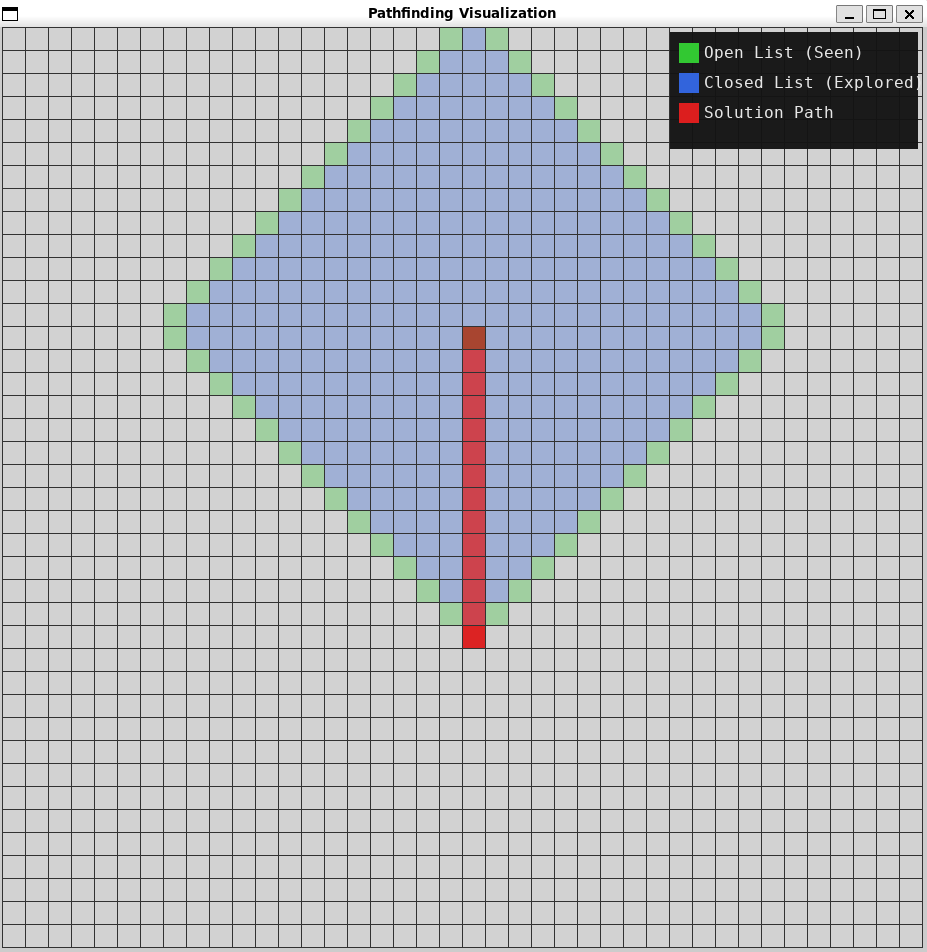
\includegraphics[width=\linewidth]{map1_bfs}}
    \centerline{\small (a) BFS}
\end{minipage}
\hfill
\begin{minipage}[b]{0.30\textwidth}
    \centerline{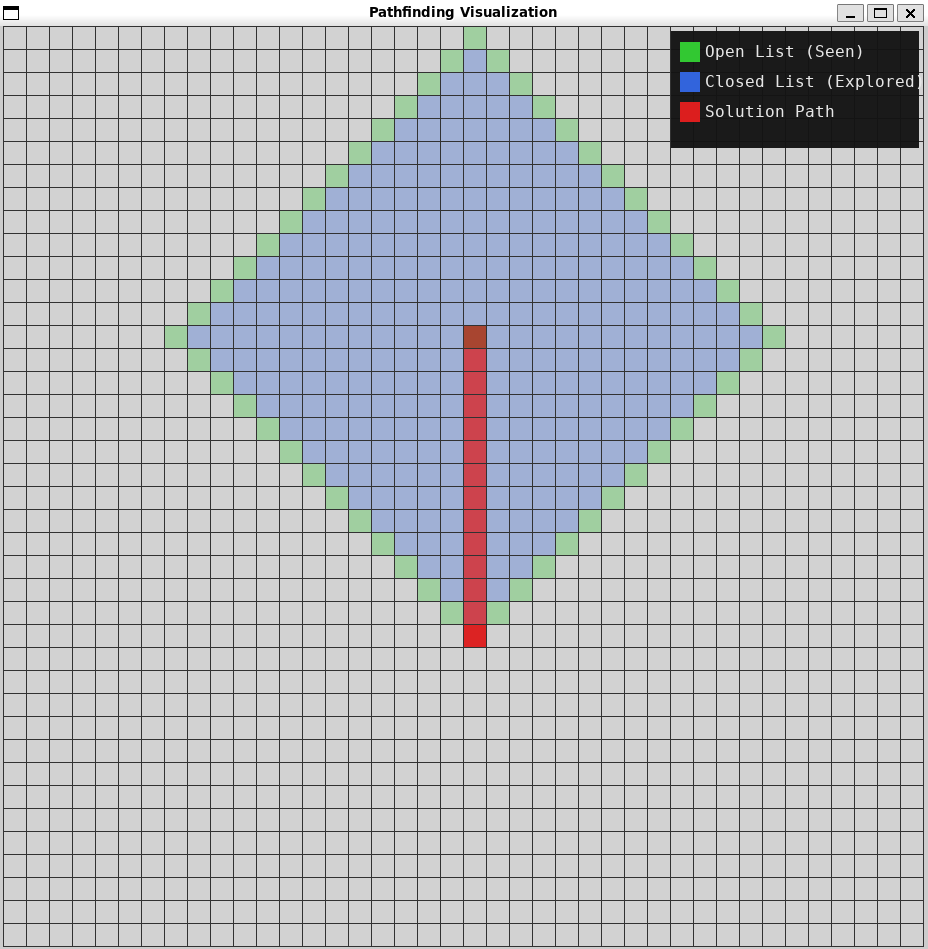
\includegraphics[width=\linewidth]{map1_ucs}}
    \centerline{\small (b) UCS}
\end{minipage}
\hfill
\begin{minipage}[b]{0.30\textwidth}
    \centerline{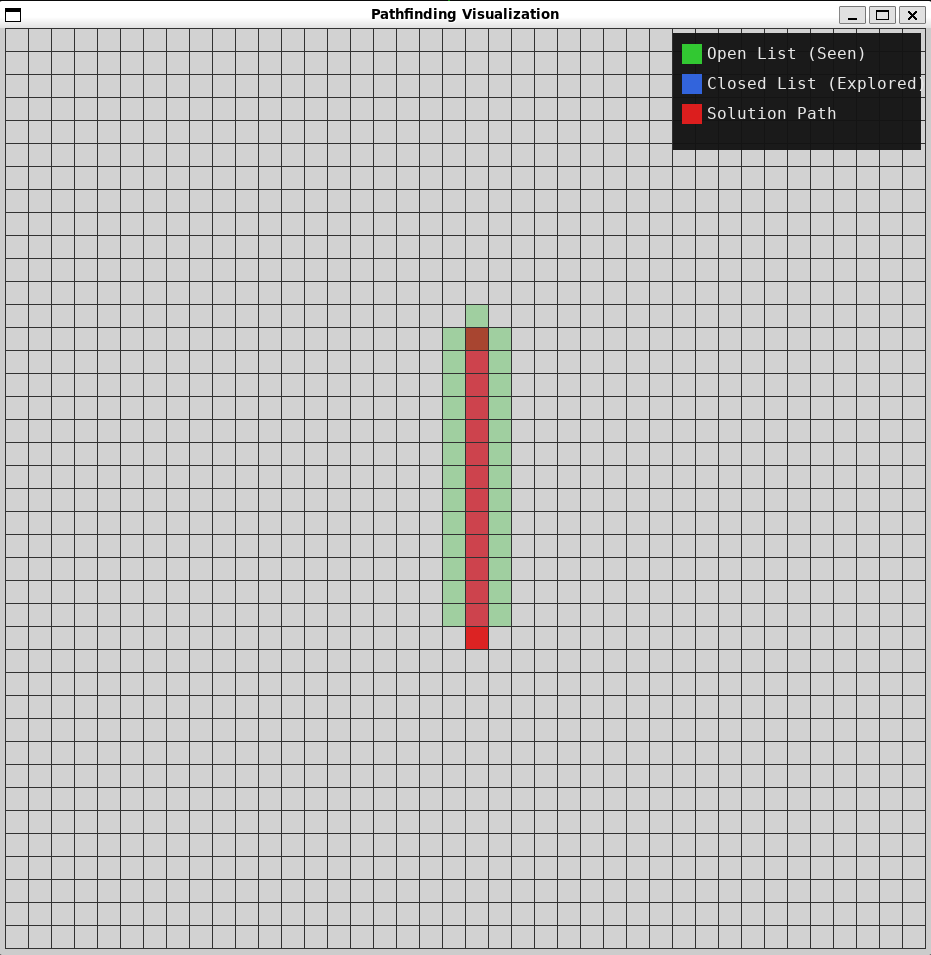
\includegraphics[width=\linewidth]{map1_gbfs}}
    \centerline{\small (c) GBFS}
\end{minipage}

\vspace{0.8em}

\begin{minipage}[b]{0.30\textwidth}
    \centerline{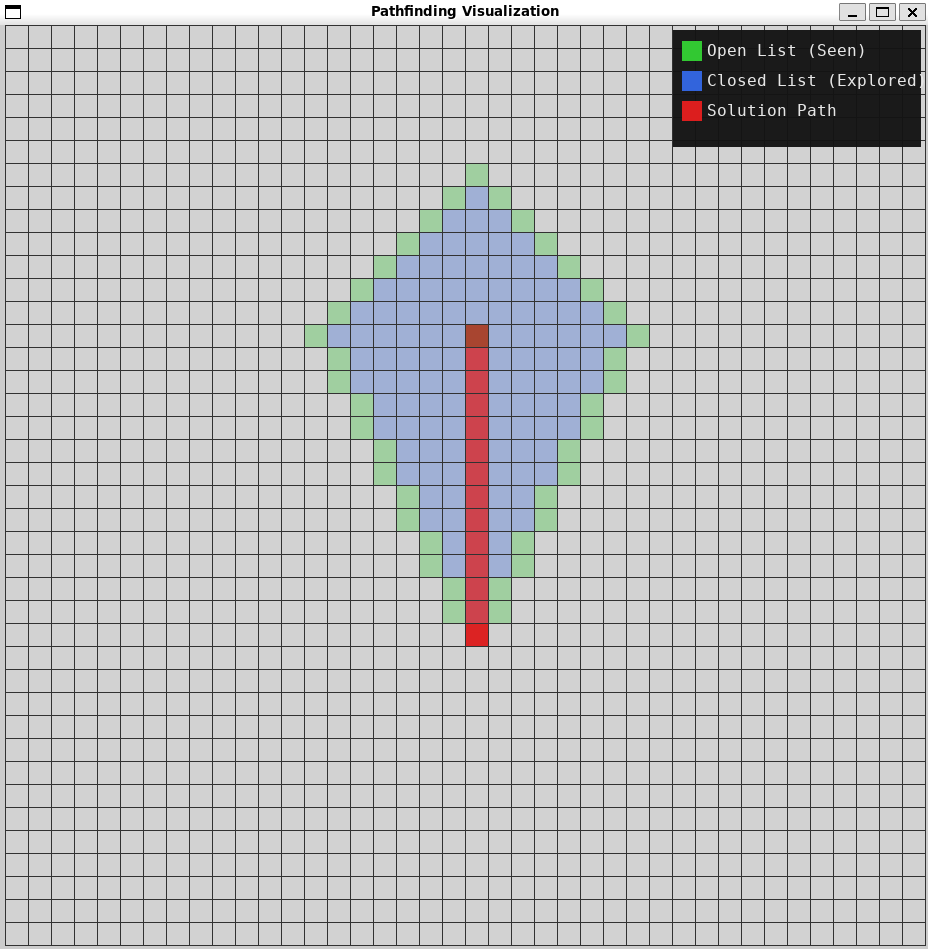
\includegraphics[width=\linewidth]{map1_astar1}}
    \centerline{\small (d) A* Heuristic 1}
\end{minipage}
\hspace{0.17\textwidth}
\begin{minipage}[b]{0.30\textwidth}
    \centerline{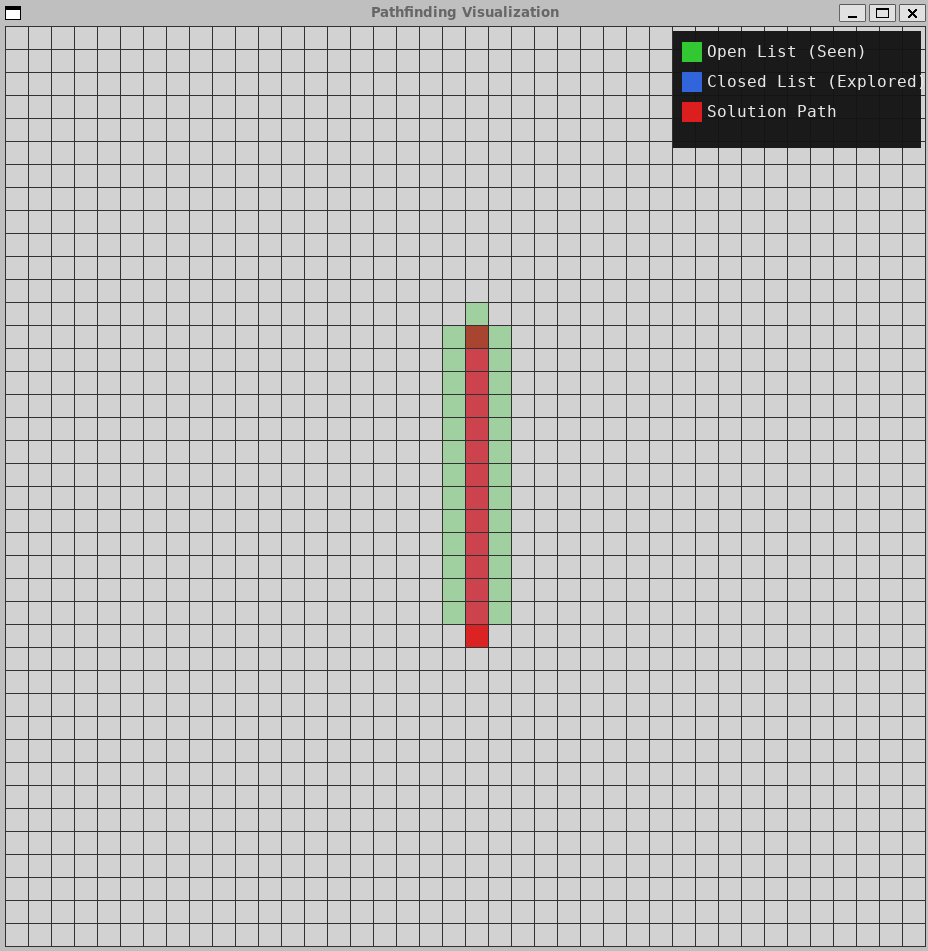
\includegraphics[width=\linewidth]{map1_astar2}}
    \centerline{\small (e) A* Heuristic 2}
\end{minipage}

\caption{Final visualization state for each algorithm on Map 1.}
\label{fig:map1}
\end{figure}

\begin{table}[H]
\caption{Map 1 --- Algorithm Analytics}
\begin{center}
\begin{tabular}{lcccc}
\toprule
\textbf{Algorithm} & \textbf{Path Length} & \textbf{Path Cost} & \textbf{Expanded Nodes} & \textbf{Seen Nodes} \\
\midrule
BFS            & 14 & 36 & 338 & 52 \\
UCS            & 14 & 36 & 331 & 51 \\
GBFS           & 14 & 36 & 13  & 27 \\
A* Heuristic 1 & 14 & 36 & 121 & 39 \\
A* Heuristic 2 & 14 & 36 & 13  & 27 \\
\bottomrule
\end{tabular}
\label{tab:map1}
\end{center}
\end{table}

% -------------------------------------------------------

\subsection{Map 2}

\begin{figure}[H]
\centering
\begin{minipage}[b]{0.30\textwidth}
    \centerline{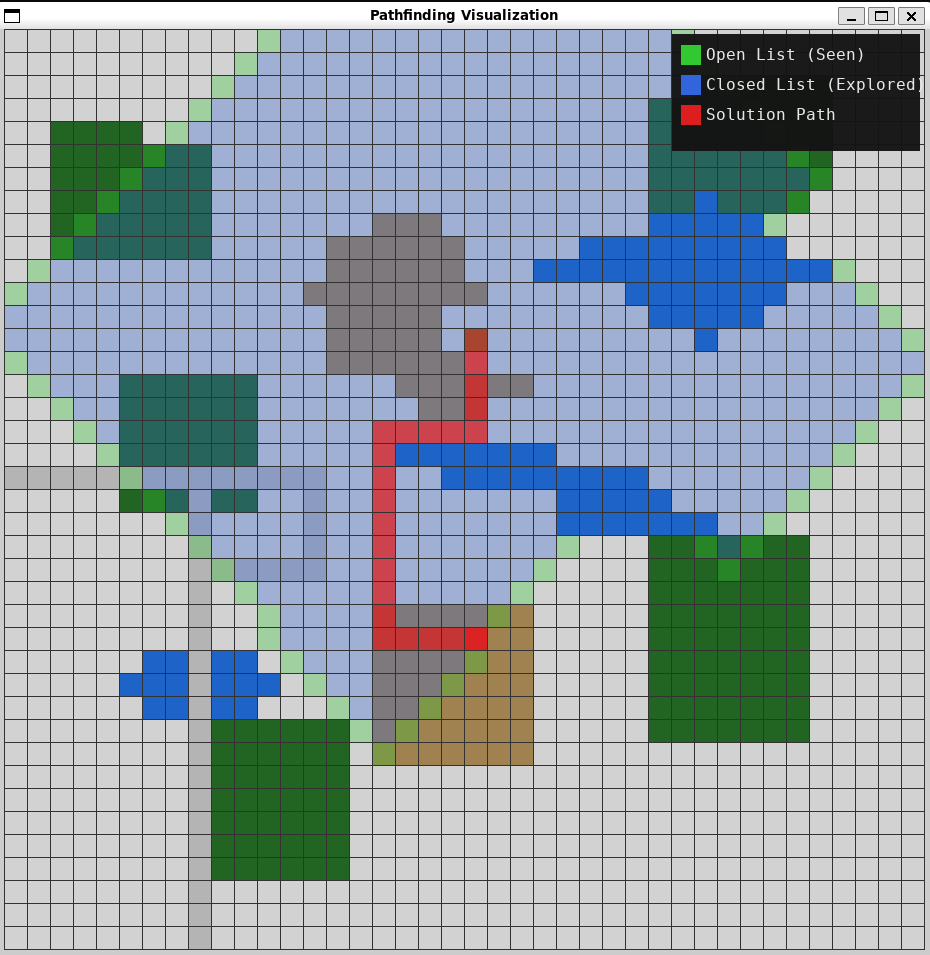
\includegraphics[width=\linewidth]{map2_bfs}}
    \centerline{\small (a) BFS}
\end{minipage}
\hfill
\begin{minipage}[b]{0.30\textwidth}
    \centerline{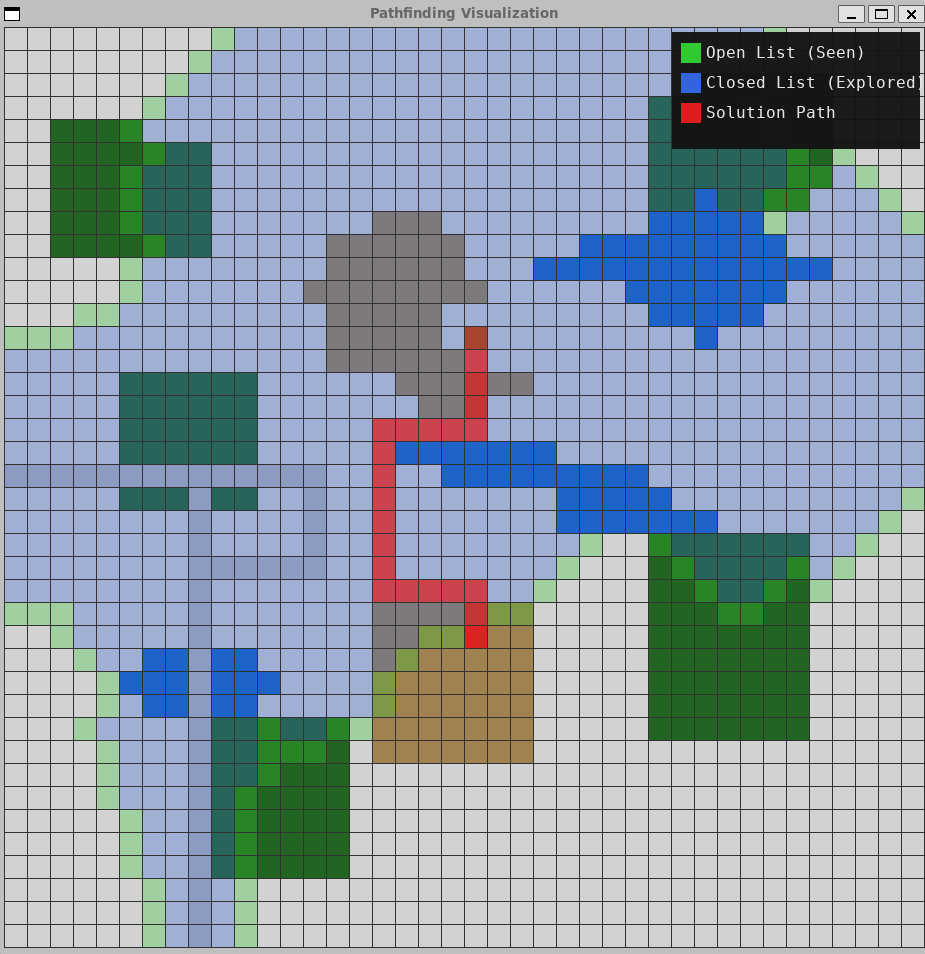
\includegraphics[width=\linewidth]{map2_ucs}}
    \centerline{\small (b) UCS}
\end{minipage}
\hfill
\begin{minipage}[b]{0.30\textwidth}
    \centerline{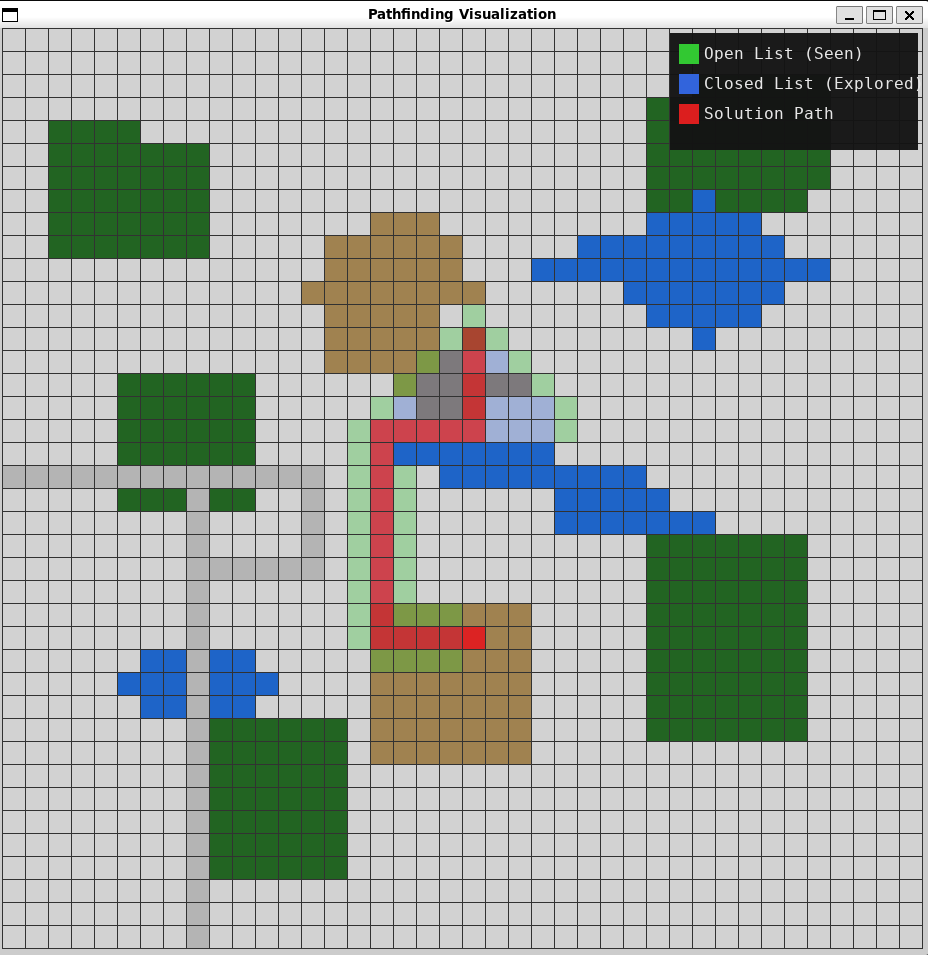
\includegraphics[width=\linewidth]{map2_gbfs}}
    \centerline{\small (c) GBFS}
\end{minipage}

\vspace{0.8em}

\begin{minipage}[b]{0.30\textwidth}
    \centerline{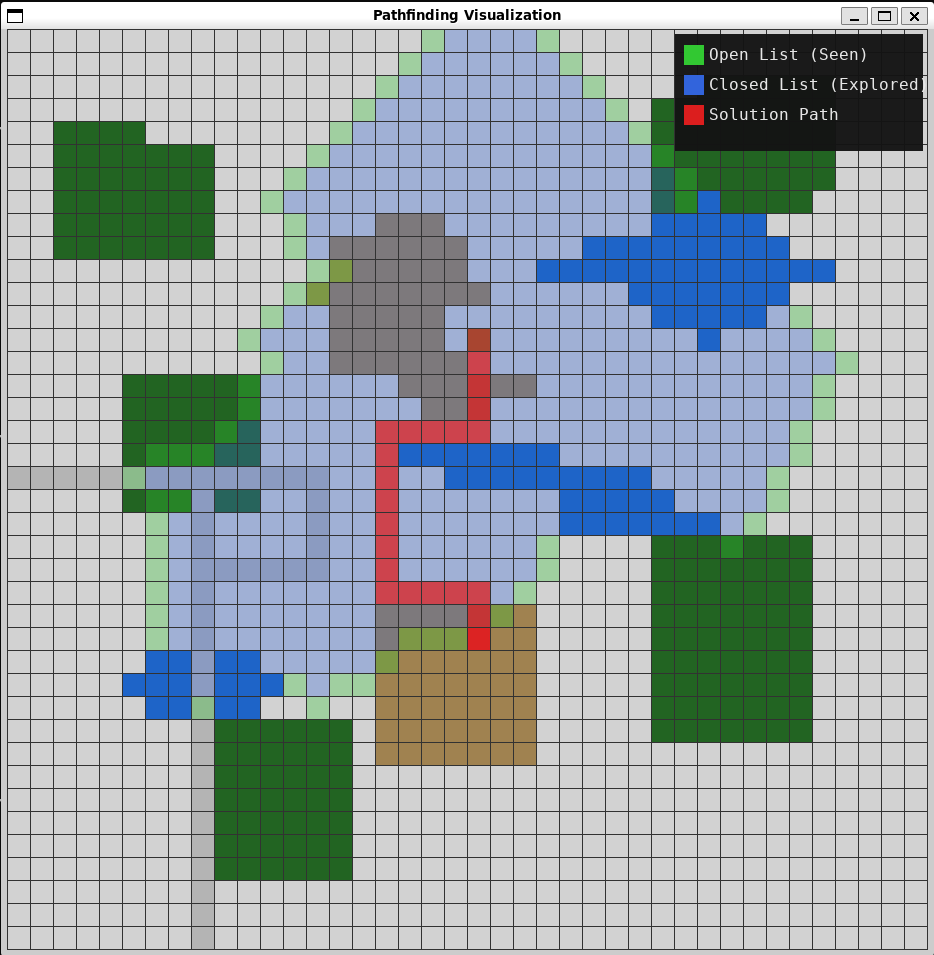
\includegraphics[width=\linewidth]{map2_astar1}}
    \centerline{\small (d) A* Heuristic 1}
\end{minipage}
\hspace{0.17\textwidth}
\begin{minipage}[b]{0.30\textwidth}
    \centerline{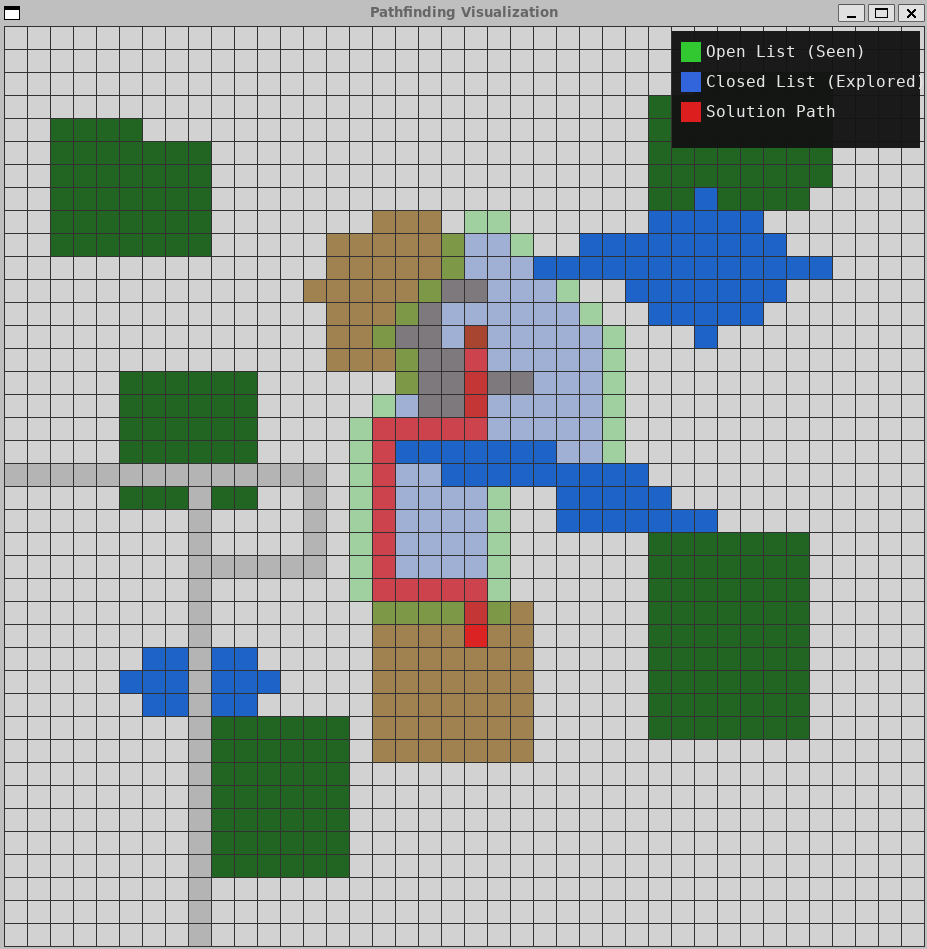
\includegraphics[width=\linewidth]{map2_astar2}}
    \centerline{\small (e) A* Heuristic 2}
\end{minipage}

\caption{Final visualization state for each algorithm on Map 2.}
\label{fig:map2}
\end{figure}

\begin{table}[H]
\caption{Map 2 --- Algorithm Analytics}
\begin{center}
\begin{tabular}{lcccc}
\toprule
\textbf{Algorithm} & \textbf{Path Length} & \textbf{Path Cost} & \textbf{Expanded Nodes} & \textbf{Seen Nodes} \\
\midrule
BFS            & 22 & 95  & 657 & 61 \\
UCS            & 22 & 75  & 852 & 85 \\
GBFS           & 22 & 95  & 36  & 33 \\
A* Heuristic 1 & 22 & 75  & 424 & 64 \\
A* Heuristic 2 & 22 & 75  & 93  & 37 \\
\bottomrule
\end{tabular}
\label{tab:map2}
\end{center}
\end{table}

% -------------------------------------------------------

\subsection{Map 3}

\begin{figure}[H]
\centering
\begin{minipage}[b]{0.30\textwidth}
    \centerline{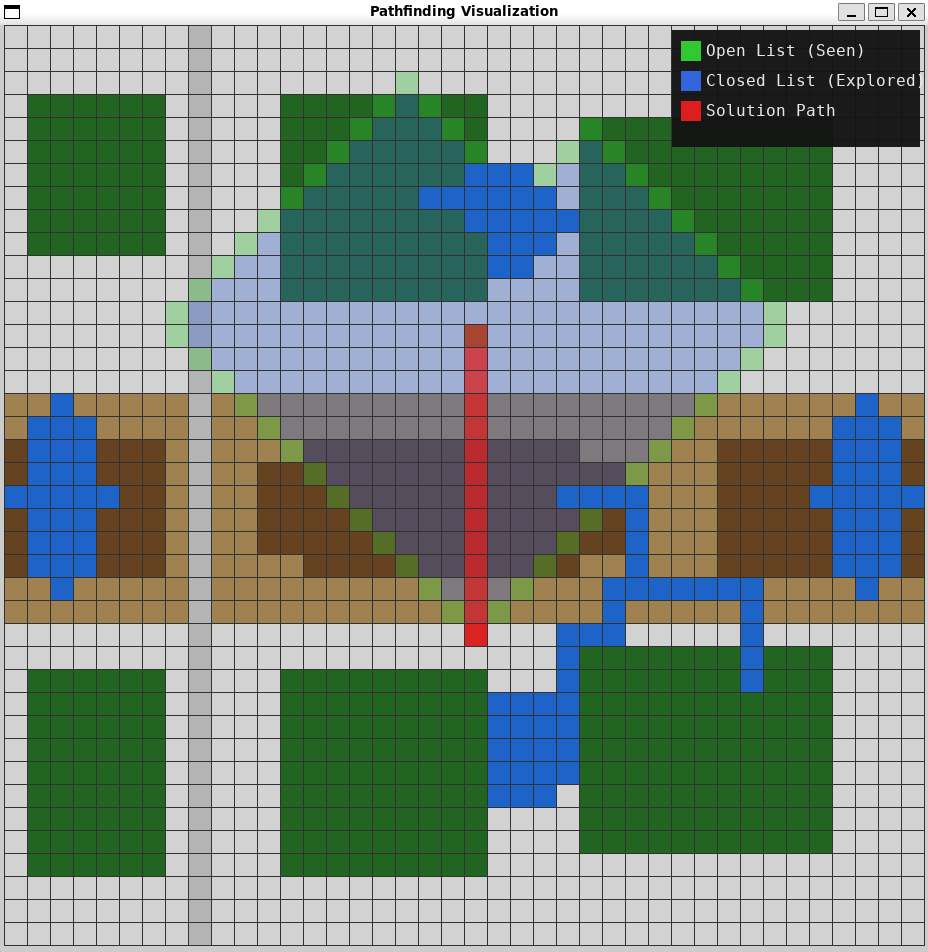
\includegraphics[width=\linewidth]{map3_bfs}}
    \centerline{\small (a) BFS}
\end{minipage}
\hfill
\begin{minipage}[b]{0.30\textwidth}
    \centerline{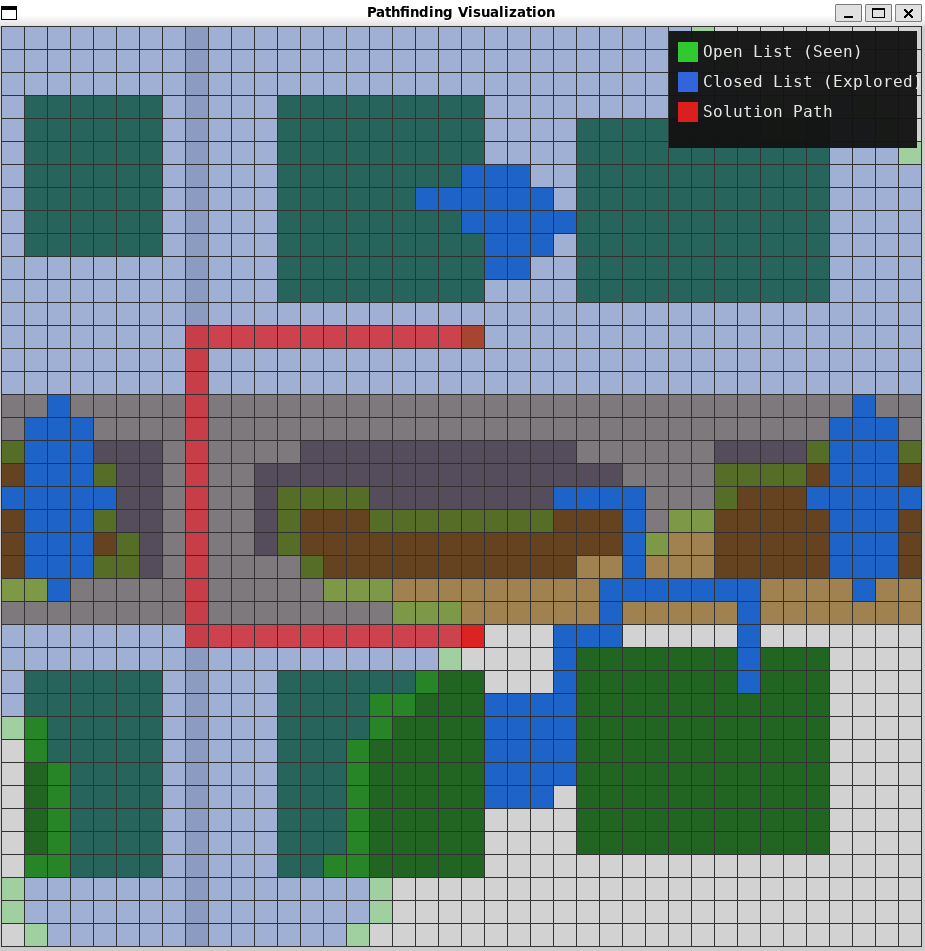
\includegraphics[width=\linewidth]{map3_ucs}}
    \centerline{\small (b) UCS}
\end{minipage}
\hfill
\begin{minipage}[b]{0.30\textwidth}
    \centerline{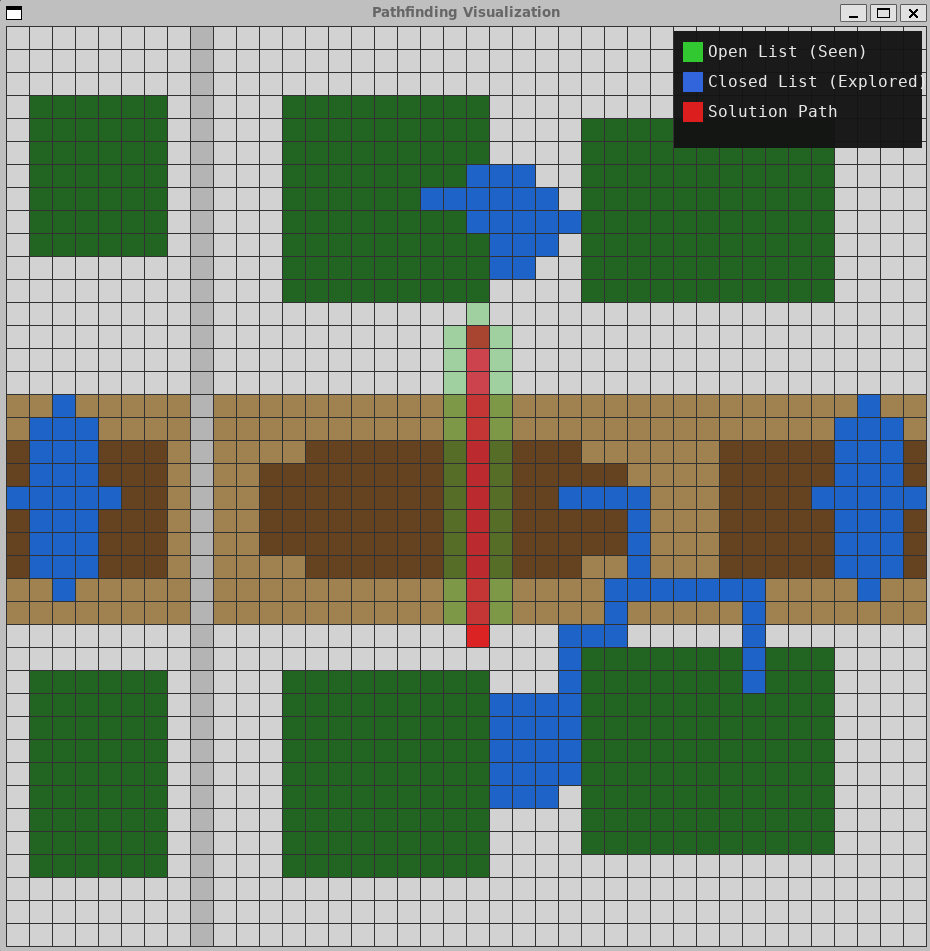
\includegraphics[width=\linewidth]{map3_gbfs}}
    \centerline{\small (c) GBFS}
\end{minipage}

\vspace{0.8em}

\begin{minipage}[b]{0.30\textwidth}
    \centerline{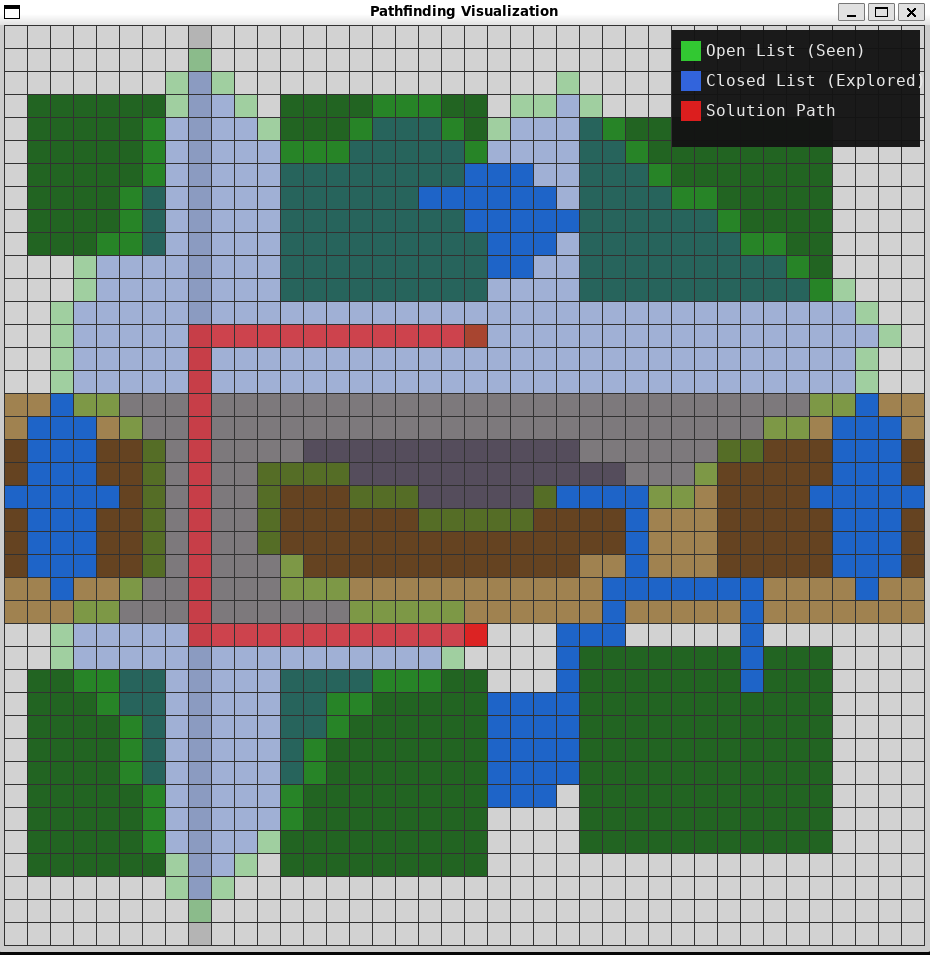
\includegraphics[width=\linewidth]{map3_astar1}}
    \centerline{\small (d) A* Heuristic 1}
\end{minipage}
\hspace{0.17\textwidth}
\begin{minipage}[b]{0.30\textwidth}
    \centerline{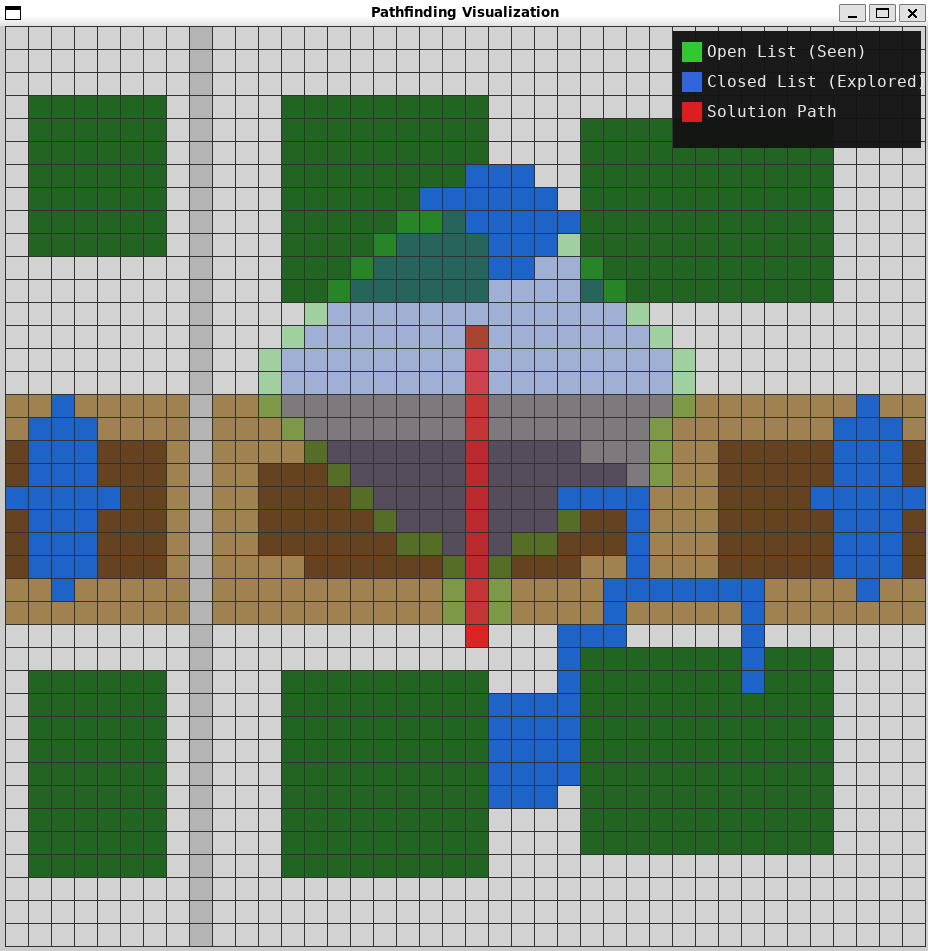
\includegraphics[width=\linewidth]{map3_astar2}}
    \centerline{\small (e) A* Heuristic 2}
\end{minipage}

\caption{Final visualization state for each algorithm on Map 3.}
\label{fig:map3}
\end{figure}

\begin{table}[H]
\caption{Map 3 --- Algorithm Analytics}
\begin{center}
\begin{tabular}{lcccc}
\toprule
\textbf{Algorithm} & \textbf{Path Length} & \textbf{Path Cost} & \textbf{Expanded Nodes} & \textbf{Seen Nodes} \\
\midrule
BFS            & 14 & 128 & 290 & 50 \\
UCS            & 38 & 80  & 981 & 77 \\
GBFS           & 14 & 128 & 13 & 27 \\
A* Heuristic 1 & 38 & 80 & 535 & 122 \\
A* Heuristic 2 & 14 & 128 & 165 & 37 \\
\bottomrule
\end{tabular}
\label{tab:map3}
\end{center}
\end{table}

% -------------------------------------------------------

\section*{Conclusion}

The results from the evaluated algorithms in this project were mostly what was expected based on their calculated $O(n)$ time and space efficiency. Due to the input being designed with Cost taken into account, BFS is almost always useless since the solution's optimality is also defined by the Cost of the found path. Except for maps like Map 1 where all the Cell's Cost were uniform. Again though this was expected due to knowing that the optimality of BFS is measured in actions to Goal state. That is not saying much though, as all 5 of the test algorithms found the optimal path for Map 1 and BFS was the least efficient of them all. At first glance it may surprise you that BFS and UCS do not have the exact same amount of Cells expanded and Cells seen, as these two algorithms are identical when the map is uniform in regards to Cost, except for the fact that BFS is the only algorithm of those evaluated that allows for duplicates on the OpenList which explains this discrepancy. Looking at the other Maps where Cost is a factor, all 5 of the algorithms on Map 2 either found the optimal solution or were close to finding it, as this Map is still simple enough that the most aggressive algorithms, Greedy Best-First Search and A* with an inadmissible heuristic are able to get the most out of their heuristics without any of the drawbacks. BFS and UCS were very inefficient compared to the other two, and when given a complex cost map UCS with its BFS like exploration thoroughness and the overhead of taking cost into consideration was the more inefficient. Despite this, it is optimal and always found the best solution even on the most complex map. GBFS was by far the most efficient algorithm, finding a solution orders of magnitude before the likes of UCS and even A* Heuristic 1. Although when faced with Map 3, its greedy approach of heuristic only guidance led it to find a solution that was very suboptimal, traversing the mountain range in a straight path. A* Heuristic 2 failed Map 3 in a similar way, as this algorithm was using a heuristic that was overestimating the road path through the pass. Leading towards branches leading over to those road cells being sorted much further back on the OpenList than they should have been. A* Heuristic 1 and UCS were the only two algorithms on Map 3 to correctly find the optimal path by taking the road through the pass, UCS able to do this by sorting each and every Cell seen by its $g$-cost at each depth level, and A* Heuristic 1 with a smarter approach of combining the admissible Manhattan heuristic with the seen Cell's $g$-cost, also allowing for it to find the path in less than half the expanded Cells. Out of curiosity I generated a perfect heuristic set, where using a reverse UCS algorithm run starting it at the End cell to get a true cost value for each Cell to the End cell, then running the Greedy Best-First Search algorithm using that heuristic instead of the Manhattan heuristic I expected it to be able to find the road and the optimal path on Map 3. Even with this perfect heuristic the GBFS due to its complete discarding of $g$-cost failed to find the road, although it did travel through the pass correctly. The heuristic value it is blindly trusting was achieved by using the road, but since GBFS does not know that this unexpected behavior is seen in the below figure.


\begin{figure}[H]
\centering
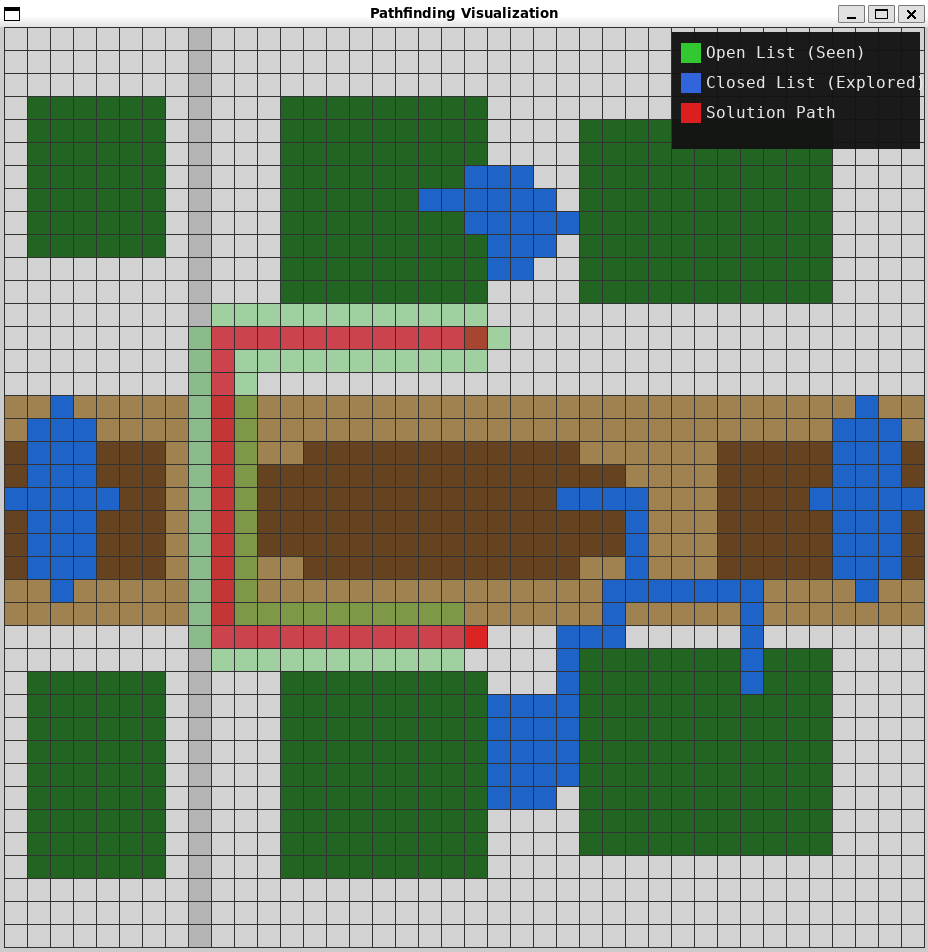
\includegraphics[width=0.6\linewidth]{map3_gbfs_perfect_heuristic}
\caption{GBFS Perfect Heuristic Fail}
\label{fig:gbfs_perfect}
\end{figure}

% -------------------------------------------------------

\section*{Use of Artificial Intelligence and LLMs}

\subsection{Coding}
Almost all of the code for this project was written by the Claude Sonnet 4.6 model. The way I acheived this was via seven different .md context files. The first of which being a general context in the root level of the repository and 6 seperate specific task definition context files. These detailed task files were where I broke down the task at hand after splitting up the work required for this project based on the architecture I settled on. Each task file contains algorithm specifics, struct and class definitions and interfaces between the different modules, classes and methods. After setting the Claude Sonnent 4.6 model onto a task I always instructed the LLM to come back to me with any questions it had that pertained to the task.md file it had just processed. Also I asked it for any suggestions and made decisions on whether it should go ahead with those suggestions. This ended up working out very well. I would then go through the edits the model came back with and wrote the comments myself. Alot of the time I would rewrite certain elements of the implementation to use python datastructures that I was more familiar with, so I could be sure that the implementation of the algorithm was how I understood and designed it. An issue with this approach was that the model was choosing different Python data-structures due to their better lookup efficiency, even though it made the algorithms implementation a bit less understandable to the human eye. Something I found very useful about this approach was I had to spend very little time understanding the pygame visualization library, leaving me more time to focus on the algorithms and their efficiencies. All of the task.md files are included in my final .tar of this projects code.

\subsection{Writing}
All of the Latex structural code that compiles into this document was generated by the same Claude Sonnet 4.6 model. In regards to the contents of each section and subsection, that is all my own words and understanding. The only use of the Sonnet 4.6 model for that content was for spelling and grammar checking.

\end{document}
